%
%	Praxisbezug
%

\pagebreak
\section{mTLS Analysis}

\onehalfspacing

\subsection{Resource Consumption}

To evaluate the two service meshes, we will look at the following Kubernetes metrics:\footnote{See \textit{Kubernetes (2023)}: Resource Pipeline. \cite{resPipeline}}

\begin{itemize}
    \item Number of pods
    \item CPU reserved
    \item CPU used
    \item Memory reserved
    \item Memory used
\end{itemize}

We will take the values from the Rancher cluster dashboard for each experiment iteration.

\begin{figure}[H]
\centering
\caption {Cluster Dashboard}
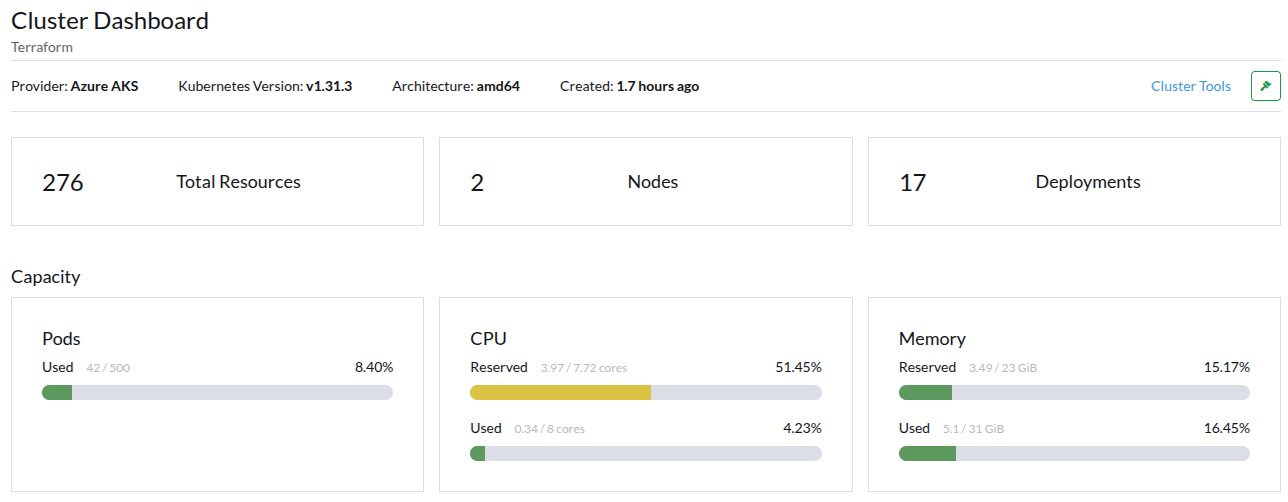
\includegraphics[width=\linewidth]{images/cluster-dashboard.png}
\label{fig:clusterDashboard}
\end{figure}

Here are the tabulated results from the experiment:

\begin{table}[ht]
  \caption{Resource Consumption}
    \begin{tabular}{| l | l | l | l | l | l |}
    \hline
    & Pods & CPU Rsvd & CPU Used & Memory Rsvd & Memory Used \\
    \hline\hline
    Idle & 37 & 3.97 cores & 0.32 cores & 3.49 GB & 4.78 GB \\
    \hline
    App Only & 42 & 3.97 cores & 0.34 cores & 3.49 GB & 5.1 GB \\
    \hline
    Linkerd & 59 & 3.97 cores & 0.61 cores & 3.49 GB & 13 GB \\
    \hline
    Istio & 61 & 5.93 cores & 1.02 cores & 7.14 GB & 13 GB \\
    \hline
    \hline
    \end{tabular}
  \label{tab:resUsage}
\end{table}

\subsection{Installation Time}

Installing the two service meshes was not very time-consuming. We measured the time from the beginning of the first command until after the Helm chart was finished installing the software.

\begin{table}[ht]
  \caption{Installation Time}
    \begin{tabular}{| l | l |}
    \hline
    & Time \\
    \hline\hline
    Linkerd & 5 min \\
    \hline
    Istio & 20 min \\
    \hline
    \hline
    \end{tabular}
  \label{tab:installTime}
\end{table}

Istio requires several prerequisites, such as a running monitoring stack, which makes the installation significantly longer.

\subsection{Enabling mTLS}

The documentation made enabling mTLS for our sample application straightforward, either from the CLI or through auto-injection. We measured the time it took to enable mTLS on the installed sample application.

\begin{table}[ht]
  \caption{Enabling mTLS}
    \begin{tabular}{| l | l |}
    \hline
    & Time \\
    \hline\hline
    Linkerd & 5 min \\
    \hline
    Istio & 5 min \\
    \hline
    \hline
    \end{tabular}
  \label{tab:enableTime}
\end{table}

There was no difference in time or effort between Istio and Linkerd regarding enabling mTLS for our sample application.

\subsection{Linkerd and Istio Evaluation}

From our experiment, we can derive the following conclusions:

\begin{itemize}
    \item Istio uses more resources and takes longer to deploy
    \item Istio and Linkerd both offer automatic traffic encryption
\end{itemize}

Further findings include:

\begin{itemize}
    \item Istio enables Metrics by default and includes its own observability console, Kiali.\footnote{See \textit{Istio (2025)}: Kiali. \cite{istioKiali}}
    \item Istio uses the Envoy proxy, a well-established industry standard
    \item Istio is available for Kubernetes clusters but can support virtual machines and bare metal environments
    \item Linkerd uses its own linkerd-2 proxy
    \item Linkerd focuses on Kubernetes clusters only
\end{itemize}

Istio offers very powerful traffic management capabilities, allowing for fine-grained control over how traffic flows through the service mesh.

Linkerd, on the other hand, is designed to be easier to install, configure, and manage than Istio. Its resource consumption above shows it's more lightweight and has a more negligible performance overhead.

In summary, Istio offers a robust and comprehensive solution for complex microservices architectures, while Linkerd prioritizes simplicity and ease of use for less demanding environments. For a complex microservices architecture with demanding traffic management and security requirements, Istio might be the better choice.

Both service meshes handle application traffic encryption equally well.

\subsection{Outlook}

So far, we've only looked at application traffic encryption. Both service meshes also allow authentication policies to restrict traffic between applications and arrive more at a zero-trust network security model.\footnote{See \textit{Gemini (2025)}: What is Zero-Trust Networking. \cite{bardZeroTrust}} 

Other options to explore in a future paper include Istio's Ingress and Egress gateways, which allow network policies to extend across clusters and include non-Kubernetes resources. Similarly to Istio, Linkerd also offers a multi-cloud feature.

Both service mesh installations that we have looked at in this paper use the sidecar injection pattern. Istio now offers with Ambient mode an option to run a service mesh without sidecars, which could be worthwhile to explore, too.\footnote{See \textit{Istio (2024)}: Istio's Ambient Mode. \cite{istioAmbient}}
